% Paper Track Writeup draft. Kaggle limit: 3,000 words. Build: make   (or: latexmk -pdf main)
% Guidance for editing is in WRITING-GUIDE.md. Red [YOU: ...] markers are the only items left for the author.
\documentclass[11pt]{article}
\usepackage[margin=1in]{geometry}
\usepackage[T1]{fontenc}
\usepackage{microtype,booktabs,xcolor,graphicx,amsmath,amssymb,enumitem}
\usepackage[hidelinks]{hyperref}
\usepackage{pgfplots}
\pgfplotsset{compat=1.18}

\newcommand{\todo}[1]{\textcolor{red}{[\textbf{YOU:} #1]}}

\title{Training-Free Rank-One Prompt Distillation for a Quantized Gemma~4 Coding Agent\\[2pt]
\large Regime boundaries, causal controls, and preserved failures}
\author{\todo{Author 1} \qquad \todo{Author 2} \qquad \todo{Author 3} \\[4pt]
\normalsize Independent Researchers}
\date{November 2026}

\begin{document}
\maketitle

\begin{abstract}
Small coding agents often fail at one step of the repair loop. We ask whether a closed-form, rank-one weight edit can carry one such behaviour---rereading source after a failed partial-line edit---into the competition's 4-bit quantized Gemma~4 E4B through its standard PEFT-adapter path, and what governs when that transfer holds or breaks. The edit uses the output shift between a prompted and an unprompted agent at one decision token, whitened by background key statistics, installed as one rank-1 component of a rank-8 adapter on layer~29 \texttt{self\_attn.o\_proj}. Under frozen, pre-registered protocols, a static-prototype edit and the activation-derived edit at unit strength ($\alpha=1$) both failed. A post-hoc diagnostic revealed why: although the whitened key fires on held-out prefixes (cosine $0.99$), a single-layer rank-1 shift at $\alpha=1$ recovers only $6\%$ of the full prompt's $+3.32$-nat log-probability margin, leaving the reread decision below the $0$-nat greedy boundary ($-0.47$~nats). With $\alpha=4$ chosen on design cases only to cross that boundary ($+0.15$~nats), the edit completed 21 and 23 of 24 target workflows in two greedy runs on fresh cases, against 4--5 for base and 0 for its sign-flipped copy, matching a gradient-trained rank-8 LoRA (24/24) within the pre-registered margin. Because greedy selection masks a thin logit margin ($+0.15$ vs.\ $+2.65$~nats for the prompt), the effect weakens under stochastic decoding: at temperature~0.7 (shared seed) one seed passed and one collapsed into empty stop-token completions; at the competition's setting (temperature~0.2, thinking enabled, independent seeds), first-action rereads dropped to roughly half the prompt's rate (22/48 vs.\ 39/48), passing all gates in batch~A (15 vs.\ 3 workflows) but missing the net-$+6$ gate in batch~B (10 vs.\ 6), even though the edit completed slightly more total workflows than the prompt (25/48 vs.\ 21/48) under the six-request thinking cap. On three real repair issues where the target error rarely arose, neither arm repaired an issue and the edit arm ran slower.
\end{abstract}

\section{Introduction}
A small coding agent pays for every instruction twice: each line of system prompt consumes context in a 32k-token window, and a small model follows the line only some of the time. In our tool-session tests the competition's baseline agent shows this cost after an edit leaves a line half-written, retrying the stale replacement instead of inspecting the file. One prompt sentence fixes that, and we ask whether the behaviour can be written into the weights without the sentence.

Weight-space programming~\cite{takehi2026} and model editing~\cite{meng2022,sun2026,mazzawi2025} suggest closed-form updates with no gradient training. Moving from single-token benchmarks to a deployed coding agent introduces four constraints rarely tested together: a 4-bit quantized checkpoint (\texttt{gemma-4-e4b-it-qat-w4a16-ct}), a standard PEFT adapter served through vLLM, a multi-step tool loop where one bad action corrupts state, and stochastic thinking-mode decoding fixed by an external scorer. We test whether one closed-form, rank-one edit can move a tool-calling decision through that stack, and map the regime boundary where rank-one distillation succeeds and where it breaks down.

\paragraph{Contributions.}
\begin{itemize}[leftmargin=*,itemsep=1pt,topsep=2pt]
\item \textbf{Causal directional transfer under greedy decoding:} A covariance-whitened rank-one edit ($\alpha=4$, chosen on design cases only) deployed as a PEFT adapter on a quantized E4B lifts target workflows from 4--5/24 (base, zero, and norm-matched random controls) to 21--23/24, matches a gradient-trained LoRA (24/24) within the pre-registered margin, and reverses to 0/24 under sign-flipping.
\item \textbf{Mechanistic diagnosis of the greedy-to-sampling gap:} A single-layer rank-one update recovers $\approx 0.20$~nats per unit of $\alpha$ against a $+3.32$-nat multi-layer prompt shift. Choosing the smallest $\alpha$ that flips greedy decoding ($\alpha=4$, mean margin $+0.15$~nats) yields near-perfect deterministic behaviour while leaving the decision near $50\%$ once stochastic sampling and intermediate thinking tokens intervene.
\item \textbf{Preserved failures and operational trade-offs:} We report two failed initial designs, a high-temperature ($T=0.7$) stop-token collapse that greedy evaluation hid, a mixed two-batch outcome under competition thinking settings (edit rereads 22/48 vs.\ prompt 39/48, yet finishes 25/48 vs.\ 21/48 workflows due to lower turn overhead), and a three-issue real harness check showing latency cost when the target fault is rare.
\end{itemize}

\section{Related work and claim boundary}\label{sec:related}
The linear algebra of rank-one updates is established and we claim none of it. ROME~\cite{meng2022} writes a key--value association into one layer with a closed-form rank-one update whitened by input covariance; our update has the same form. Steer2Edit~\cite{sun2026} converts contrasting-response steering vectors into training-free rank-one edits of attention-head output projections and MLP neurons using weight-derived keys; we edit \texttt{self\_attn.o\_proj} but take the key and covariance from activations. Mazzawi et al.~\cite{mazzawi2025} turn a prompt's effect into token-independent updates via a closed-form least-squares solve over activations on Gemma~3 1B MLP weights; our output shift is likewise a prompted-minus-unprompted difference. Yin et al.~\cite{yin2026} compile a steering vector into a persistent closed-form weight change under a null-space constraint as a backdoor attack. Gradient-trained LoRA distillation is the standard alternative, which we run as a baseline.

What prior works do not characterize, as far as we could find, is how closed-form rank-one prompt distillation behaves across the deployment gap of a quantized, multi-turn tool agent: shipping the edit as a PEFT adapter on a 4-bit quantized checkpoint through vLLM, separating directional steering from perturbation via sign-flipped controls, and measuring how thin single-layer logit margins interact with stochastic sampling and thinking-mode rollouts. We do not test blind weight reading or the broader claims of~\cite{takehi2026}.

\section{Method}\label{sec:method}
\subsection{Target behaviour}
After an edit leaves a syntax error, the base agent repeats a stale replacement; a prompt saying ``reread, then replace the whole line'' makes it call \texttt{read\_file} first. At the decision token, 12/12 design cases reread under that prompt and 0/12 under base. Cases are seeded synthetic tool sessions (an arithmetic \texttt{adjust} function) checked by a restricted interpreter and the official editor; a workflow is complete only if the final source is correct, tested after the last edit, and submitted.

\subsection{Construction}
On 12 design cases we replay each history under both prompts and record, at the last token before the tool call, the input $k$ and output $o$ of \texttt{self\_attn.o\_proj} in layers 12--38. Let $d$ be the mean prompted-minus-base output and $k^\ast$ the mean base input; the layer maximizing $\lVert d\rVert/\lVert\bar o_{\text{base}}\rVert$ is used (layer~29, width 4096). A ridge-regularized covariance $C$ over all tokens of 12 non-target design cases whitens the key, so the edit responds to what is distinctive about the target state and stays near zero on ordinary inputs:
\begin{equation}
\Delta W \;=\; \alpha\,\frac{d\,(C^{-1}k^\ast)^{\top}}{k^{\ast\top}C^{-1}k^\ast},\qquad \Delta W\,k^\ast=\alpha\,d .
\end{equation}
It is installed as one rank-1 component of a rank-8, $\alpha_{\text{LoRA}}=8$ bf16 adapter ($0.17\%$ shift error). The strength $\alpha$ is the smallest value in $\{2,3,4,6,8\}$ for which greedy decoding on design cases rereads in at least 11/12 target cases and leaves the first tool call unchanged in all 12/12 non-target cases ($\alpha=4$). No evaluation case enters design or selection.

\subsection{Controls, baseline, and frozen protocols}
We compare six arms: unchanged \textbf{base}; \textbf{zero adapter} ($B=0$); seeded \textbf{random adapter} with matched factor norms; \textbf{sign-flipped edit} ($\alpha=-4$); the instruction \textbf{prompt}; and a \textbf{gradient-trained LoRA} baseline (rank-8 on the same module, trained on the 24 design cases with the prompted continuation as teacher and preservation targets on non-target cases, stopped at step~40 upon meeting the design-set rule). Adapter application in vLLM was verified separately: active adapters shift first-token log-probabilities by 0.09--0.76~nats on three fixed prefixes with 0.0~nats zero-control drift. Every experiment was frozen before inference, with cases, gates, and budgets hashed in a ledger; evaluation cases use disjoint coefficient pairs never seen in design.

\section{Results}\label{sec:results}
\subsection{Failures first and the logit-margin mechanism}
Two initial designs failed their pre-registered gates. A static-prototype edit built from token embeddings completed 9/12 workflows on a development screen versus 10/12 for base and 12/12 for the prompt (4/24 in the full panel). Next, the activation-derived edit at $\alpha=1$ (36 fresh cases, 8 arms, 288 trajectories) completed 3/24 target workflows versus 4/24 for base, with 0/24 first-action rereads, even though vLLM checks confirmed first-token shifts of 0.09--0.27~nats.

A post-hoc diagnostic on those 24 evaluation prefixes explained why $\alpha=1$ produced zero behavioural change despite firing cleanly. On held-out prefixes, the whitened key fires with mean dot product $0.99$ (cosine $0.9995$), and the teacher-forced margin $\Delta \ell = \log P(\texttt{read\_file}) - \log P(\texttt{edit\_file})$ grows monotonically with $\alpha$ (versus $+2.65$~nats for the prompt):
\[
\Delta \ell(\alpha):\quad
\underbrace{-0.85}_{\alpha=-1} \;<\;
\underbrace{-0.67}_{\alpha=0\text{ (base)}} \;<\;
\underbrace{-0.47}_{\alpha=1} \;<\;
\underbrace{-0.29}_{\alpha=2} \;<\;
\underbrace{+0.15}_{\alpha=4} \;<\;
\underbrace{+0.91}_{\alpha=8}\;\text{nats.}
\]
Because the prompt acts across all layers and positions, it shifts $\Delta\ell$ by $+3.32$~nats ($-0.67$ to $+2.65$~nats). A single-layer shift at $\alpha=1$ adds $+0.20$~nats ($\approx 6\%$ of the prompt's shift), leaving $\Delta \ell < 0$ on all 24 cases (0/24 rereads). At $\alpha=4$, the mean margin crosses zero to $+0.15$~nats (22/24 cases $>0$). That diagnostic motivated the design-set strength grid and is a disclosed researcher degree of freedom.

\subsection{Greedy decoding on fresh cases (\texorpdfstring{$\alpha=4$}{alpha = 4})}
With $\alpha=4$ selected on design cases only, we ran two pre-registered greedy panels on 36 fresh cases: Run~1 (6 arms, 216 trajectories) tested perturbation controls, and Run~2 (5 arms, 180 trajectories) tested the gradient-trained LoRA (Table~\ref{tab:greedy}).

\begin{table}[ht]
\centering
\caption{Greedy evaluation on 36 fresh cases ($\alpha=4$). Non-target workflows were 12/12 in every arm. A dash means the arm was not run.}
\label{tab:greedy}
\vspace{2pt}
\begin{tabular}{lrrrr}
\toprule
 & \multicolumn{2}{c}{First action = \texttt{read\_file} (of 24)} & \multicolumn{2}{c}{Workflows complete (of 24)} \\
\cmidrule(lr){2-3} \cmidrule(lr){4-5}
Arm & Run 1 & Run 2 & Run 1 & Run 2 \\ \midrule
base & 0 & 0 & 5 & 4 \\
zero adapter & 0 & -- & 5 & -- \\
random, norm-matched & 0 & -- & 4 & -- \\
\textbf{edit ($\alpha=4$)} & \textbf{20} & \textbf{22} & \textbf{21} & \textbf{23} \\
sign-flipped edit ($\alpha=-4$) & 0 & 0 & 0 & 0 \\
gradient-trained LoRA & -- & 24 & -- & 24 \\
prompt & 24 & 24 & 24 & 24 \\ \bottomrule
\end{tabular}
\end{table}

Run~1 passed all four pre-registered gates: the edit beat base, zero, and random controls by net $+16$, $+16$, and $+17$ target workflows (one-sided exact sign tests, $p<10^{-4}$), beat the sign-flipped edit by $+21$ ($p=4.8\times 10^{-7}$), and lost zero non-target cases. The random control perturbed token log-probabilities more strongly than the edit (0.47--0.76 vs.\ 0.19--0.26~nats) yet produced 0 rereads and 4 completions, while the sign-flipped edit eliminated even base's occasional successes (4--5 down to 0). Run~2 repeated the pattern: under the frozen comparability rule (within 3 workflows), the edit (23/24) is comparable to the gradient-trained LoRA (24/24, trained in $\sim$5 minutes). Identical adapters gave 21 and 23 across runs ($\pm 2$ serving noise in temperature-0 vLLM batching).

\subsection{Sampling at temperature 0.7 and stop-token collapse}
At temperature~0.7 without thinking, seed~101 passed (edit 24/24 complete and 24/24 rereads, base 18/24, sign-flipped 6/24, prompt 24/24). Seed~102 was cancelled at 63/144 rows (incomplete). Seed~103 failed: edit dropped to 4/24 while base reached 24/24, sign-flipped 0/24, and prompt 24/24. Trace inspection revealed two findings: (1)~\textbf{Stop-token collapse:} in 20/24 target cases under seed~103, the $\alpha=4$ edit's first completion was empty (one token, finish reason \texttt{stop}), a side effect hidden by greedy decoding; and (2)~\textbf{Shared-seed correlation:} because all requests in a v3 batch shared one RNG seed across similar prefixes, each seed acted nearly as one draw per arm (allowing base to hit 24/24 and edit to hit 20/24 empty stops on seed~103).

\subsection{Competition setting: temperature 0.2 with thinking and independent seeds}
To fix the shared-seed flaw and test the competition regime, we froze protocol~v4: 36 new cases, temperature~0.2, \texttt{top\_p}~0.95, thinking enabled, \emph{independent per-trajectory seeds}, two batches (seeds 201 and 202, 144 trajectories each), and the same $\alpha=4$ edit with no re-tuning (Table~\ref{tab:v4}).

\begin{table}[ht]
\centering
\caption{Competition setting (temperature 0.2, thinking enabled, independent seeds). Non-target completions were 11/12 for edit in both batches versus 12/12 and 11/12 for base.}
\label{tab:v4}
\vspace{2pt}
\begin{tabular}{lrrrrrrrr}
\toprule
 & \multicolumn{4}{c}{First action = \texttt{read\_file} (of 24)} & \multicolumn{4}{c}{Workflows complete (of 24)} \\
\cmidrule(lr){2-5} \cmidrule(lr){6-9}
Batch & base & edit & sign-flip & prompt & base & edit & sign-flip & prompt \\ \midrule
A (seed 201) & 6 & \textbf{12} & 2 & 18 & 3 & \textbf{15} & 2 & 10 \\
B (seed 202) & 5 & \textbf{10} & 3 & 21 & 6 & \textbf{10} & 4 & 11 \\ \midrule
Pooled (of 48) & 11 & \textbf{22} & 5 & 39 & 9 & \textbf{25} & 6 & 21 \\ \bottomrule
\end{tabular}
\end{table}

Batch~A passed every gate: edit beat base by net $+12$ workflows ($p=0.0002$) and sign-flipped by $+13$, with one non-target loss. Batch~B moved in the same direction (10 vs.\ 6 base and 4 sign-flipped) but missed the net-$+6$ gate ($+4$, $p=0.17$), making the protocol outcome \textbf{mixed}. No empty completions occurred (0/48). Table~\ref{tab:v4} shows two effects under thinking-mode sampling:
\begin{itemize}[leftmargin=*,itemsep=1pt,topsep=2pt]
\item \textbf{Dilution of first-action steering:} On the immediate \texttt{read\_file} decision, the strict ordering sign-flipped (5/48) $<$ base (11/48) $<$ edit (22/48) $<$ prompt (39/48) holds in both batches, but the edit's reread rate drops from $\sim 88\%$ in greedy to $46\%$. An edit calibrated at the pre-generation token with a $+0.15$-nat margin loses roughly half its pull once stochastic sampling and intermediate \texttt{<think>} tokens intervene before the tool call.
\item \textbf{Turn-budget trade-off vs.\ the prompt:} Despite fewer first-action rereads (22/48 vs.\ 39/48), the edit completed slightly \emph{more} workflows than the prompt (25/48 vs.\ 21/48; 15 vs.\ 10 in batch~A). Between 8 and 15 of 24 trajectories per arm ended on the six-request budget, which caps completions when thinking mode consumes turns.
\end{itemize}

\begin{figure}[ht]
\centering
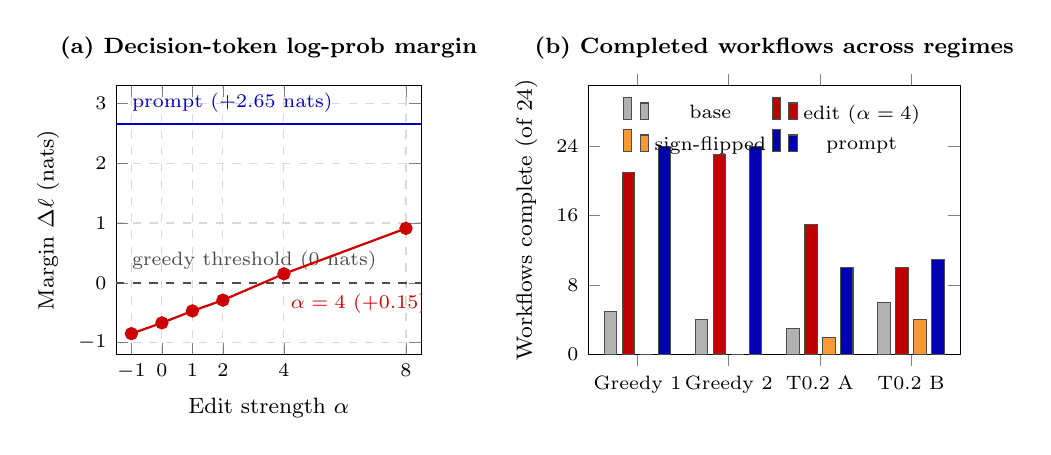
\begin{tikzpicture}
\begin{axis}[
    name=leftplot,
    width=0.45\linewidth,
    height=5.0cm,
    xlabel={Edit strength $\alpha$},
    ylabel={Margin $\Delta\ell$ (nats)},
    xmin=-1.5, xmax=8.5,
    ymin=-1.2, ymax=3.3,
    xtick={-1,0,1,2,4,8},
    ytick={-1,0,1,2,3},
    tick label style={font=\scriptsize},
    label style={font=\footnotesize},
    title style={font=\footnotesize\bfseries},
    title={(a) Decision-token log-prob margin},
    grid=major,
    grid style={dashed,gray!30}
]
\addplot[thick, black!70, dashed, domain=-1.5:8.5] {0};
\addplot[thick, blue!75!black, domain=-1.5:8.5] {2.65};
\node[font=\scriptsize, blue!75!black, anchor=south west] at (axis cs:-1.3,2.68) {prompt ($+2.65$~nats)};
\node[font=\scriptsize, black!70, anchor=south west] at (axis cs:-1.3,0.05) {greedy threshold ($0$~nats)};
\addplot[thick, mark=*, mark size=2pt, red!80!black] coordinates {
    (-1,-0.85) (0,-0.67) (1,-0.47) (2,-0.29) (4,0.15) (8,0.91)
};
\node[font=\scriptsize, anchor=north west, red!80!black] at (axis cs:3.9,-0.02) {$\alpha=4$ ($+0.15$)};
\end{axis}

\begin{axis}[
    at={(leftplot.outer north east)},
    anchor=outer north west,
    xshift=0.25cm,
    ybar,
    width=0.52\linewidth,
    height=5.0cm,
    bar width=4.5pt,
    ymin=0, ymax=31,
    ytick={0,8,16,24},
    ylabel={Workflows complete (of 24)},
    symbolic x coords={Greedy 1,Greedy 2,T0.2 A,T0.2 B},
    xtick=data,
    tick label style={font=\scriptsize},
    label style={font=\footnotesize},
    title style={font=\footnotesize\bfseries},
    title={(b) Completed workflows across regimes},
    legend style={font=\scriptsize,at={(0.5,0.98)},anchor=north,legend columns=2,draw=none,fill=none},
    enlarge x limits=0.18
]
\addplot[fill=gray!60,draw=black!70] coordinates {(Greedy 1,5)(Greedy 2,4)(T0.2 A,3)(T0.2 B,6)};
\addplot[fill=red!75!black,draw=black!70] coordinates {(Greedy 1,21)(Greedy 2,23)(T0.2 A,15)(T0.2 B,10)};
\addplot[fill=orange!80,draw=black!70] coordinates {(Greedy 1,0)(Greedy 2,0)(T0.2 A,2)(T0.2 B,4)};
\addplot[fill=blue!70!black,draw=black!70] coordinates {(Greedy 1,24)(Greedy 2,24)(T0.2 A,10)(T0.2 B,11)};
\legend{base,edit ($\alpha=4$),sign-flipped,prompt}
\end{axis}
\end{tikzpicture}
\caption{\textbf{(a)} Teacher-forced first-action margin $\Delta\ell = \log P(\texttt{read\_file}) - \log P(\texttt{edit\_file})$ across $\alpha$. Choosing $\alpha=4$ crosses the $0$-nat greedy threshold ($+0.15$~nats) but leaves a much thinner margin than the prompt ($+2.65$~nats). \textbf{(b)} Completed target workflows (of 24) across valid independent runs.}
\label{fig:overview}
\end{figure}

\subsection{Worked example}\label{sec:example}
One target case from batch~A (multiply by $-3$, add~2) illustrates both directional repair and turn-budget overhead. An earlier partial-line edit left line~2 as
\begin{quote}\small\texttt{return (-3 * value) + (2)urn (-3 * value) + (0)}\end{quote}
and the test reports a syntax error. Base does not inspect the file: it calls \texttt{edit\_file} three times with the stale line as \texttt{old\_string}, corrupts line~1, and exhausts its budget with the file broken. With the $\alpha=4$ edit, the first call is \texttt{read\_file}; the second replaces the corrupted line; the test passes and the patch is submitted in four calls. The sign-flipped edit makes four blind replacements and submits a broken file. The prompted agent also rereads first and fixes the file, but spends all six requests deliberating before submitting. Five of the 24 target cases in batch~A follow this pattern.

\subsection{A first check inside the official repair harness}\label{sec:real}
Finally, we froze a breakage protocol on real issues: the unchanged competition agent against the same agent with the $\alpha=4$ edit on its root model, on three qualified \texttt{Rich} issues (\texttt{rich\_4077}, \texttt{rich\_3772}, \texttt{rich\_3521}) in the official harness at competition settings, one sampled trajectory per issue (Table~\ref{tab:real}).

\begin{table}[ht]
\centering
\caption{Three real \texttt{Rich} issues in the official harness, one trajectory per arm. Tool counts include the sub-agent.}
\label{tab:real}
\vspace{2pt}
\begin{tabular}{lrr}
\toprule
Metric & base & edit ($\alpha=4$) \\ \midrule
Issues resolved (of 3) & 0 & 0 \\
Trajectories ending on the 3-minute session limit & 0 & 2 \\
Total tool calls / \texttt{read\_file} calls & 29 / 10 & 37 / 16 \\
Edits rejected by the editor / followed by a reread & 1 / 1 & 4 / 3 \\
Empty model responses & 0 & 0 \\ \bottomrule
\end{tabular}
\end{table}

Neither arm repaired an issue (an earlier base draw repaired 1/3, within single-draw variation). The adapter was verified active in vLLM (0.19--0.26~nat shifts, zero drift). Consistent with the synthetic panels, the edit arm called \texttt{read\_file} more often (16 vs.\ 10), but because the target fault was rare here---base met one rejected edit and reread after it unprompted---extra reading cost time without repair benefit: two edit trajectories hit the 3-minute limit and one ended without a testable patch, flagged as operational harm by our frozen rule.

\section{Limitations}
\begin{itemize}[leftmargin=*,itemsep=1pt,topsep=2pt]
\item \textbf{Task and template scope:} Positive evidence comes from one synthetic repair pattern in one template family (coefficient variation only). Non-target cases are at ceiling (12/12 across arms), limiting side-effect sensitivity. The three-issue \texttt{Rich} check is a single-draw breakage screen, and base ran without LoRA serving enabled (verified at 0.0~nat drift against a zero adapter).
\item \textbf{Decoding and budget constraints:} In v4, the 4,096-token thinking budget was approximated via an 8,192-token output limit, and the six-request cap truncates 8--15 of 24 thinking trajectories per arm. Temperature-0 vLLM batching carries $\pm 2$ workflow serving variance.
\item \textbf{Design degrees of freedom:} The strength grid ($\alpha \in \{2,3,4,6,8\}$) was motivated by the post-hoc margin diagnostic after $\alpha=1$ failed, though $\alpha=4$ was chosen strictly on design cases before generating v3/v4 test cases. The gradient LoRA used untuned hyperparameters, and we did not ablate numerical weight access during design.
\end{itemize}

\section{Reproducibility}
Protocols, case generators, adapter builders, ledger, and SHA-256-hashed reports are in the repository. Runs used Modal A10G GPUs with the competition's pinned wheels and the approved checkpoint (\texttt{gemma-4-e4b-it-qat-w4a16-ct} v2) for under USD~6 of metered compute in total (USD~4.85 across v2--v4 plus USD~0.70 for the real-issue check), conducted independently without institutional compute or funding. Operational incidents are logged: a lost terminal summary event in v2 (recomputed from streamed rows with unit-tested code), a seed-101 timeout at 196/432 rows, a report-path collision requiring seed~103, and the cancelled seed-102 batch.

\section{Conclusion}
A single closed-form, covariance-whitened rank-one weight edit, shipped as a standard PEFT adapter, installs a multi-step tool-recovery behaviour into a 4-bit quantized Gemma~4 E4B under greedy decoding---lifting completions from 4--5/24 to 21--23/24, matching a gradient-trained LoRA (24/24), and reversing to 0/24 under sign-flipping. At the same time, our diagnostic and multi-regime evaluation show why greedy success does not automatically translate to production agents: selecting the minimum strength that crosses the $0$-nat greedy boundary ($\alpha=4$, $+0.15$~nats) leaves a thin margin that loses half its pull under stochastic thinking-mode rollouts and can induce stop-token collapse at high temperature ($T=0.7$). For practitioners today, a plain prompt or a 5-minute gradient LoRA remains more reliable; making training-free rank-one edits competitive under stochastic reasoning will require calibrating strength directly under thinking-mode rollouts and gating the adapter so it activates only when an edit error occurs.

\bibliographystyle{plain}
\bibliography{references}
\end{document}
